%
% Complete documentation on the extended LaTeX markup used for Insight
% documentation is available in ``Documenting Insight'', which is part
% of the standard documentation for Insight.  It may be found online
% at:
%
%     http://www.itk.org/

\documentclass{InsightArticle}

\usepackage[dvips]{graphicx}
\usepackage{subfigure}
\usepackage{amssymb}

%%%%%%%%%%%%%%%%%%%%%%%%%%%%%%%%%%%%%%%%%%%%%%%%%%%%%%%%%%%%%%%%%%
%
%  hyperref should be the last package to be loaded.
%
%%%%%%%%%%%%%%%%%%%%%%%%%%%%%%%%%%%%%%%%%%%%%%%%%%%%%%%%%%%%%%%%%%
\usepackage[dvips,
bookmarks,
bookmarksopen,
backref,
colorlinks,linkcolor={blue},citecolor={blue},urlcolor={blue},
]{hyperref}


%  This is a template for Papers to the Insight Journal. 
%  It is comparable to a technical report format.

% The title should be descriptive enough for people to be able to find
% the relevant document. 
\title{A Spline-Driven Image Slicer}

% 
% NOTE: This is the last number of the "handle" URL that 
% The Insight Journal assigns to your paper as part of the
% submission process. Please replace the number "1338" with
% the actual handle number that you get assigned.
%
\newcommand{\IJhandlerIDnumber}{xxxx}

% Increment the release number whenever significant changes are made.
% The author and/or editor can define 'significant' however they like.
\release{0.00}

% At minimum, give your name and an email address.  You can include a
% snail-mail address if you like.
\author{J\'er\^ome Velut}
\authoraddress{jerome.velut@gmail.com}

\begin{document}

%
% Add hyperlink to the web location and license of the paper.
% The argument of this command is the handler identifier given
% by the Insight Journal to this paper.
% 
\IJhandlefooter{\IJhandlerIDnumber}


\ifpdf
\else
   %
   % Commands for including Graphics when using latex
   % 
   \DeclareGraphicsExtensions{.eps,.jpg,.gif,.tiff,.bmp,.png}
   \DeclareGraphicsRule{.jpg}{eps}{.jpg.bb}{`convert #1 eps:-}
   \DeclareGraphicsRule{.gif}{eps}{.gif.bb}{`convert #1 eps:-}
   \DeclareGraphicsRule{.tiff}{eps}{.tiff.bb}{`convert #1 eps:-}
   \DeclareGraphicsRule{.bmp}{eps}{.bmp.bb}{`convert #1 eps:-}
   \DeclareGraphicsRule{.png}{eps}{.png.bb}{`convert #1 eps:-}
\fi


\maketitle


\ifhtml
\chapter*{Front Matter\label{front}}
\fi


% The abstract should be a paragraph or two long, and describe the
% scope of the document.
\begin{abstract}
\noindent
In this article, a spline driven image slicer algorithm is presented. It is
concretized through a vtkAlgorithm-inherited class that takes two inputs and
gives two outputs. The first input is the volume from which the slice should
reconstructed while the second one is the spline which tangent vector is used as
slicing plane normal. The first output is a 2D image resliced from the volume.
The second input gives the geometric information of the slice plane location in
the volume space. An example of use is given through a simulation of a dental
panoramic view from a MDCT volume. A straightened curved planar reformation is
also applied on vascular images.
\end{abstract}

\IJhandlenote{\IJhandlerIDnumber}

\tableofcontents
%
Slicing through volume data is a common task in scientific visualization. Lots
of existing image processing tools provide this necessary functionality as soon
as the visualization of 3D (or more) data has to be performed on a 2D screen.

In VTK, different ways are possible, depending on the particular slicing needed
by the end-user. The simplest is vtkExtractVOI if the desired slice is parallel
to the input image axes. This method is used in ParaView in the Slice 
Representation. The most sophisticated is the vtkImageReslice filter in which
the cutting plane may be oriented arbitraly in the volume space. 

The algorithm presented here aims at computing the slicing orientation of a
vtkImageReslice filter directly from an input spline curve. This orientation
is defined as the Frenet-Serret frame at each point of the spline. In the 
following, a Frenet-Serret variant is proposed in order for the spline tangents
to be used as slice plane normals. An application on mandibule panoramic 
visualisation is presented, as well as an implementation of the Straightened
Curved Planar Reformation in vascular imaging.
%
\section{Frenet-Serret frame along a curve}
Frenet \cite{FRE52} and Serret \cite{SER51} defined independently several
properties on non degenerate curves from the euclidean space. Though the 
Frenet--Serret formulas aim to describe moving particles, they may be of
interest for defining local charts in a 3D space. 
%
\subsection{Initial definition}
%
Let $\mathcal{C}$ be a continuous differentiable curve in the euclidean space
$\mathbb{R}^3$ parameterized by $t$. Each point of $\mathcal{C}$ has $(x,y,z)$
coordinates. The Frenet--Serret frame of $\mathcal{C}$ at $t$ is made of the 
tangent $T$, normal $N$ and binormal $B$ unit vectors with:
\begin{eqnarray}
T(t) &=& \frac{d\mathcal{C}(t)}{dt}\label{eq:tangent}\\
N(t) &=& \frac{dT(t)}{dt}\label{eq:normal}\\
B(t) &=& T(t)\times N(t)\label{eq:binormal}
\end{eqnarray}
%
Figure~\ref{fig:frenet-serret_frames} shows such frames along a closed curve
in $3D$-space. It is important to note that equations~\eqref{eq:tangent}--\eqref{eq:binormal}
define a set of charts without taking into account the curvature and torsion of
the curve. In the following, only discrete curves are concerned. Central
differences are used to compute derivatives, constant padding is used at
boundaries and curvilinear abscissae $t$ becomes a discrete point index $k$.
%
\begin{figure}
\centering
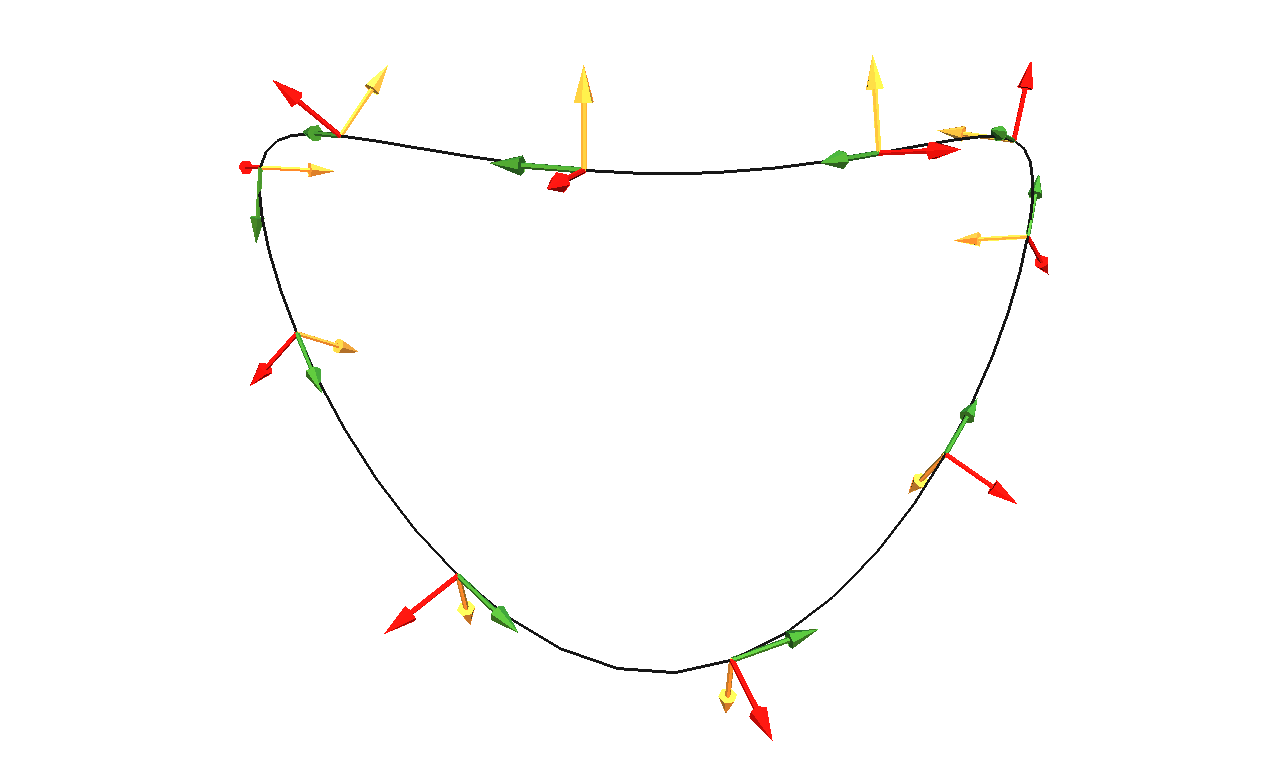
\includegraphics[width=0.7\textwidth]{Images/frenet-serret_frames}
\caption{Frenet-Serret frames along a curve: Tangents $T$ are green arrows,
Normals $N$ are red and Binormals $B$ are yellow.}
\label{fig:frenet-serret_frames}
\end{figure}
%
\subsection{Coherent consecutive normals computation}
%
The normals of a curve have the property to be directed according to the 
center of curvature. A corollary is that when the curvature changes its sign,
the normal will flip. Figure~\ref{fig:sin_normals:fs} illustrates this 
behaviour.
%
\begin{figure}
\centering
\subfigure[Frenet--Serret frames]{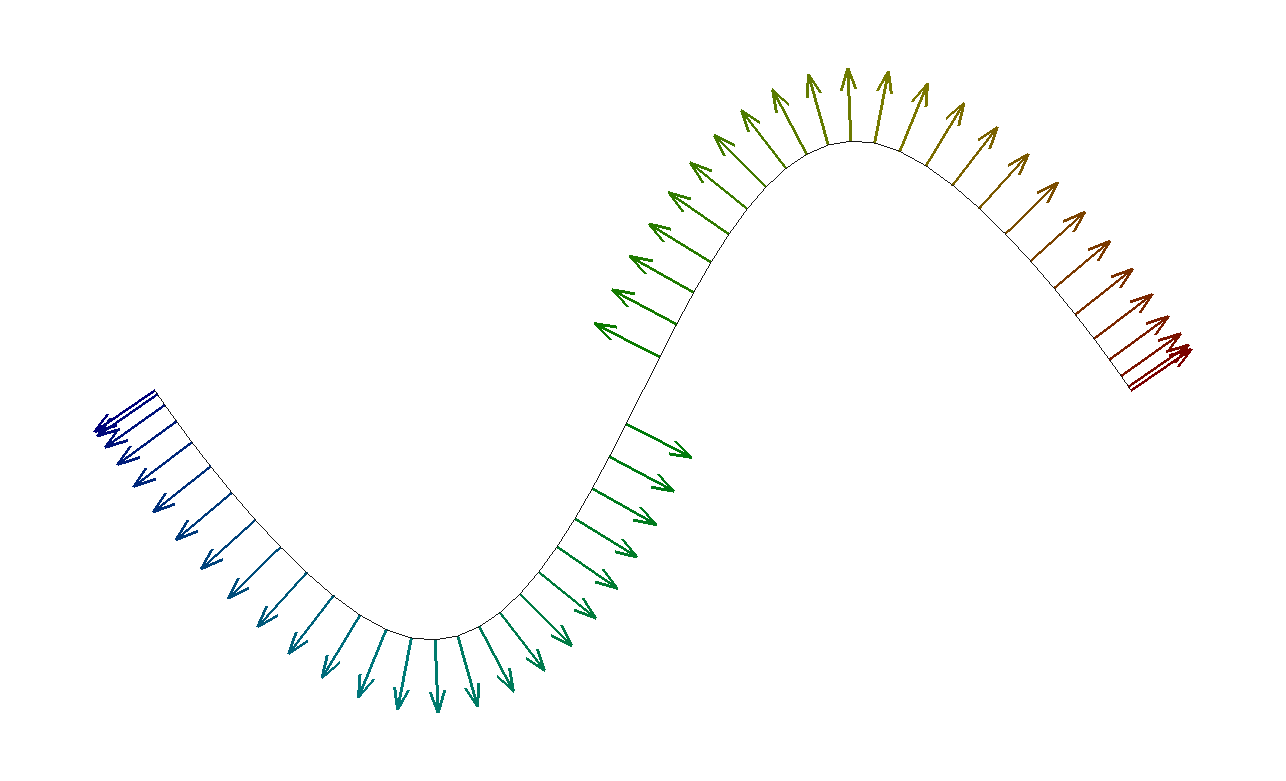
\includegraphics[width=0.5\textwidth]{Images/sin_normals_fs}\label{fig:sin_normals:fs}}
\subfigure[Enforcing consistent direction of normals]{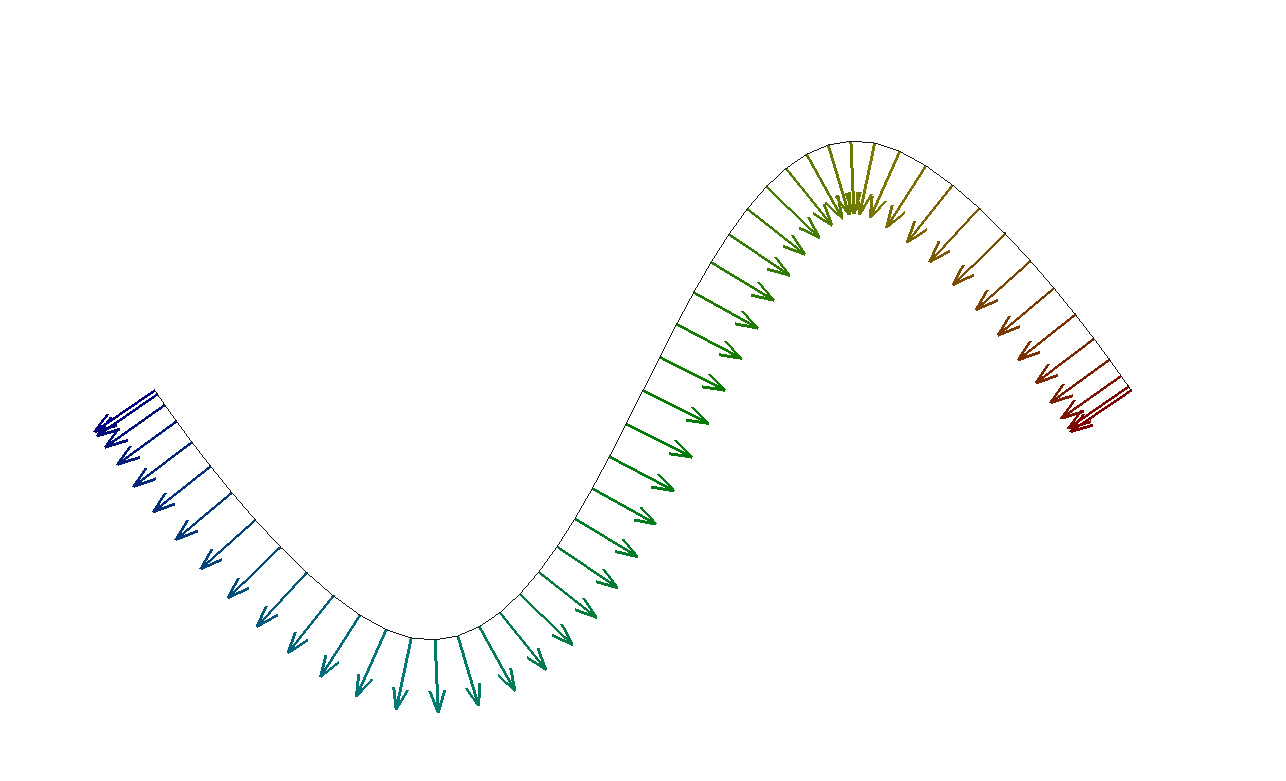
\includegraphics[width=0.5\textwidth]{Images/sin_normals_consistent}\label{fig:sin_normals:consistent}}
\caption{Normals of a curve. (a) The mathematical definition of normal induces
a change of orientation of the normal. The point where curvature is $0$ has 
null normal. (b) Arbitrary enforcing normals orientation brings consistency
along the curve.}
\end{figure}
%
As the purpose of this paper is to propose a volume slicer along a spline, the
consequence will be an annoying flip of two consecutive image slices at 
inflection points. In order to avoid that, the previous normal $N_{k-1}$ is
used to determine the current one $N_k$. The main idea is to find a projection 
of $N_{k-1}$ in the plane orthogonal to $\mathcal{C}$ at $k$. This projection
is obtained thanks to the cascaded cross product:
%
\begin{eqnarray}
B_k &=& N_{k-1} \times T_k \label{eq:consistent_binormal}\\ 
N_k &=& T_k \times B_k \label{eq:consistent_normal}
\end{eqnarray}
%
where $T_k$ is the tangent at point $k$. In 
equation~\eqref{eq:consistent_binormal}, $B_k$ represents a consistent binormal
regarding the previous one. It is not the binormal \textit{stricto sensus} as
it is computed from the previous consistent normal $N_{k-1}$, which is in turn
not the derivative of $T$ but defined in equation~\eqref{eq:consistent_normal}.

Figure~\ref{fig:sin_normals:consistent} shows that the consistent normals are
not changing their orientation at inflection points. Moreover, at the exact
inflection point, the consistent normal is not null as opposed to the 
conventional computation (figure~\ref{fig:sin_normals:fs}). A slightly 
different approach was presented in \cite{KLO86.1}.
%
\subsection{VTK implementation}
%
The Frenet-Serret frame computation along a spline is implemented in a class
\verb!vtkFrenetSerretFrame! that inherits from \verb!vtkPolyDataAlgorithm!.
The input has to be a \verb!vtkPolyData! containing at least one polyline. The 
output is a deep copy of the input plus two (optionnaly three) vector arrays, 
\verb!FSTangents! and \verb!FSNormals! (optionnally \verb!FSBinormals!). The
consistent computation is an option \verb!ConsistentNormalsOn/Off!.

According to the formulation of consistent normal vectors, they are not related
to curvature anymore. It also implies that the initial direction will be used
as a reference for the next normals. This initial direction can be arbitrary
set through the \verb!ViewUp! option.

This filter is available in ParaView by setting \verb!BUILD_PARAVIEW_PLUGIN! to
\verb!ON! during the CMake process.
%
\section{Image slicing}
%
The algorithm that extracts a 2D slice from a volume harnesses the previous
\verb!vtkFrenetSerretFrame! filter and the native VTK filter 
\verb!vtkImageReslice!. Both are connected and embedded in 
\verb!vtkSplineDrivenImageSlicer!, the latter offering an interface for the
formers' parameters.
%
\subsection{Inputs}
%
Port 0 of \verb!vtkSplineDrivenImageSlicer! is a vtkImageData port. It will be
processed by the internal \verb!vtkImageReslice! filter.

Port 1 is vtkPolyData port. The polydata must contain one or more polylines and
will serve the input of the internal \verb!vtkFrenetSerretFrame! filter.
%
\subsection{Parameters}
%
The parameters of \verb!vtkSplineDrivenImageSlicer! are related to the two main
algorithms. Table~\ref{tab:parameters} summarizes these parameters.
%
\begin{table}
\centering
 \begin{tabular}{lp{10cm}}
Name & Description \\
\hline
SliceExtent & Number of pixels in $x$ and $y$ of the output slice \\
SliceSpacing & Size of pixels in $x$ and $y$ of the output slice \\
SliceThickness & z-Spacing of the output slice, useful if appending the output to other slices \\
\hline
OffsetLine & Index of the cell in the \verb!Lines! input along which to extract the slice \\
OffsetPoint & Index of the point in the selected spline input that will represent the center of the output slice \\
Incidence & Correspond to the \verb!ViewUp! parameter of the \verb!vtkFrenetSerretFrame! filter \\
\hline
ProbeInput & Specify if the filter should or not probe the input data on the output plane 
 \end{tabular}
\caption{List of parameters of vtkSplineDrivenImageSlicer }
\label{tab:parameters}
\end{table}
%
\subsection{Outputs}
%
This algorithm provides two output ports. Output port 0 is a 
\verb!vtkImageData! representing a slice of the input volume, orthogonal to the
input spline at the specified location (\verb!OffsetLine! and 
\verb!OffsetPoint!). Image 
extent is $[0, \verb!SliceExtent![0], 0, \verb!SliceExtent![1], 0, 1]$. 
Image spacing is 
$[\verb!SliceSpacing![0], \verb!SliceSpacing![1], \verb!SliceThickness!]$. 
An additional output
is provided on output port 1 with the geometry of the slice plane.
It is a \verb!vtkPolyData! representing a grid with same resolution and size as
the output slice but oriented and centered in $\mathbb{R}^3$ according to the 
parameters, the spline and the Frenet-Serret frame. The option 
\verb!ProbeInput! allows for probing the input volume with this grid.
%
\subsection{ParaView plugin}
%
A ParaView plugin is possibly built to enable the 
\verb!vtkSplineDrivenImageSlicer!. The \verb!OffsetPoint! parameter is
animateable as well as the \verb!Incidence! parameter. For illustration, the
DICOM data INCISIX from Osirix website \cite{OSIRIX,INCISIX} are sliced along
a manually traced spline. The data represent a mandibule, the spline is chosen
to go through the teeth (figure~\ref{fig:mandibule_spline}). 
Figure~\ref{fig:mandibule_slices} have been obtained by connecting two 
spline-driven slicers to the volume and the spline (\verb!spline2.vtp!).
%
\begin{figure}
\centering
\subfigure[Volume rendering]{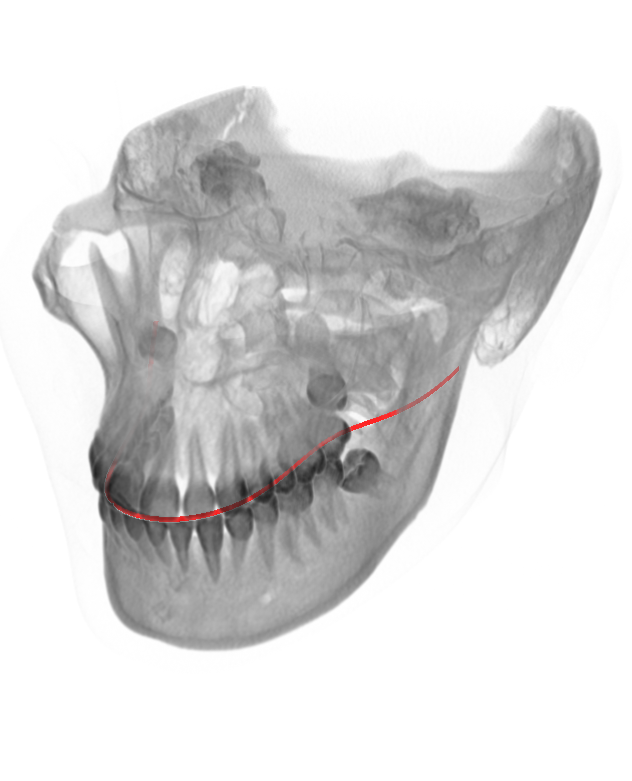
\includegraphics[width=0.35\textwidth]{Images/mandibule_spline-3d}}
\subfigure[Axial slice]{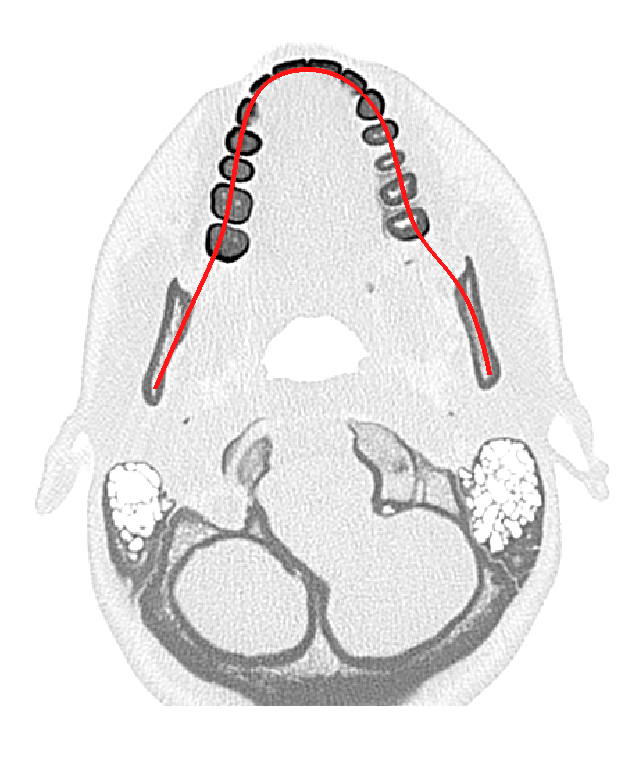
\includegraphics[width=0.35\textwidth]{Images/mandibule_spline-2d}}
\caption{Visualization from ParaView of a mandibule CT scan and a spline}
\label{fig:mandibule_spline}
\end{figure}
%
\begin{figure}
\centering
\subfigure[Slice at 150th point]{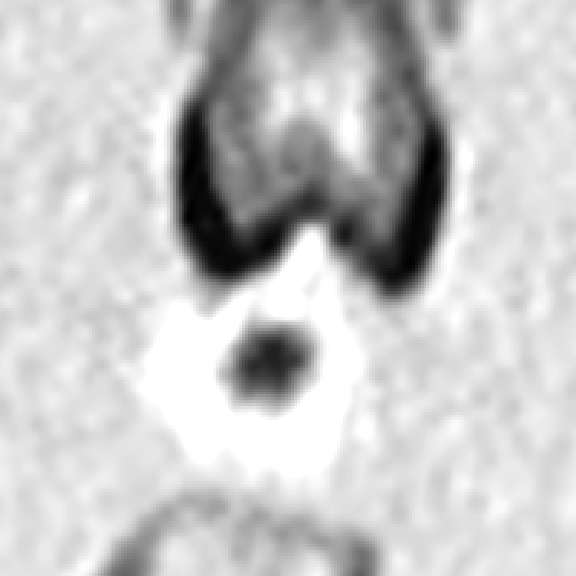
\includegraphics[width=0.24\textwidth]{Images/mandibule_slicer_offset150}}
\subfigure[Volume rendering with slice planes]{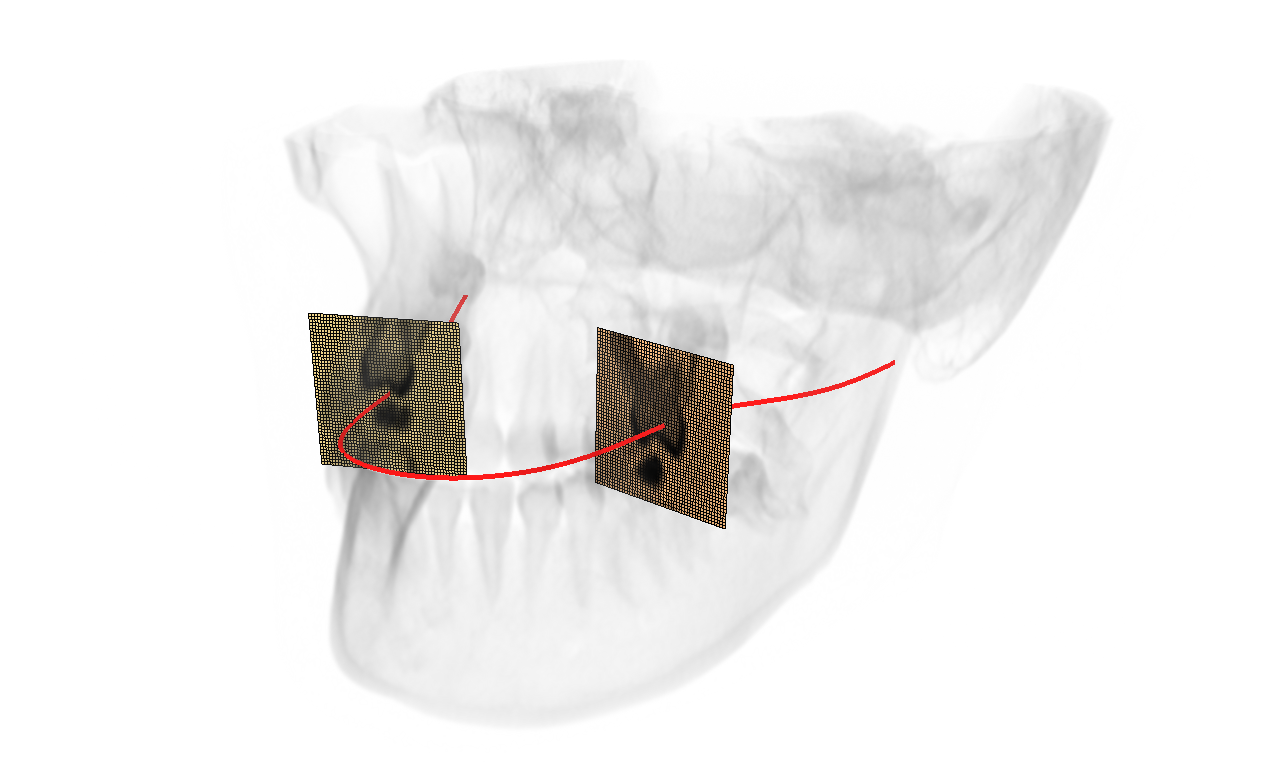
\includegraphics[width=0.5\textwidth]{Images/mandibule_2_slicers-3d}}
\subfigure[Slice at 350th point]{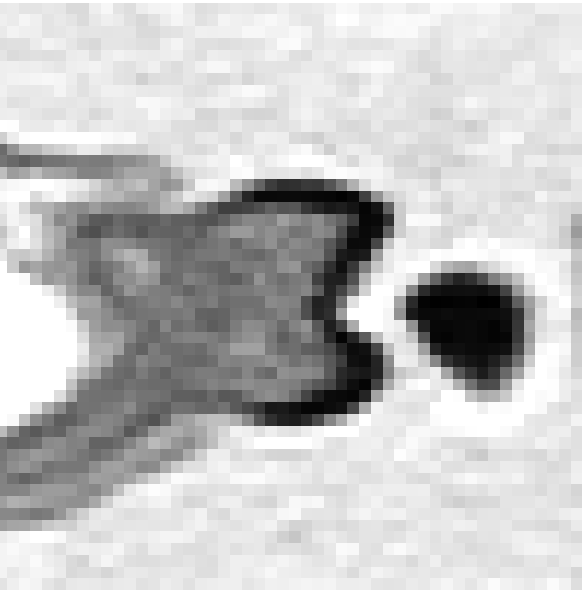
\includegraphics[width=0.24\textwidth]{Images/mandibule_slicer_offset350}}
\caption{Two slices of dimension $200\times200$, spacing $0.1\times0.1$ and
incidence $2\pi/3$}
\label{fig:mandibule_slices}
\end{figure}
%
%
\section{Straightened Curved Planar Reformation}
%
\cite{KAN01}
%
\subsection{Dental panoramic visualisation}
\begin{figure}
\centering
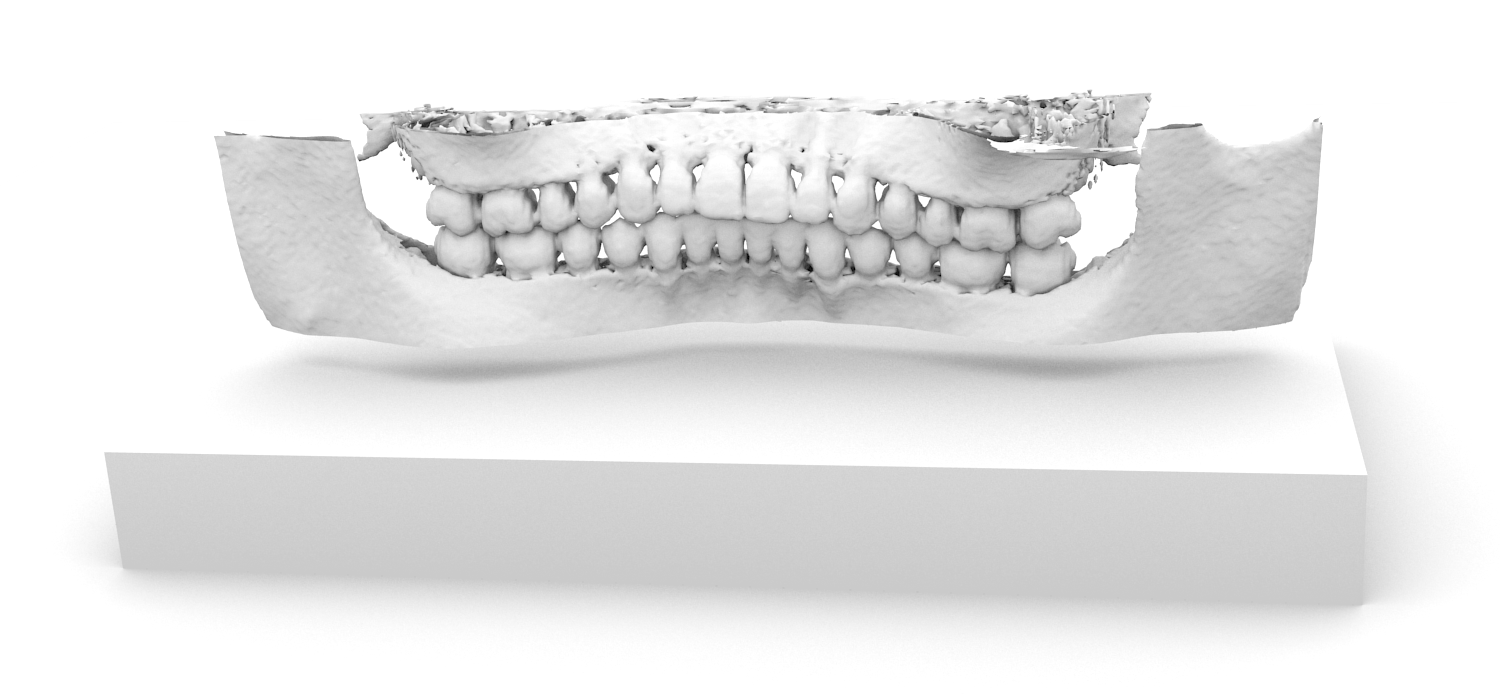
\includegraphics[width=0.8\textwidth]{Images/pano_blender.png}
\end{figure}
%
\begin{figure}
\centering
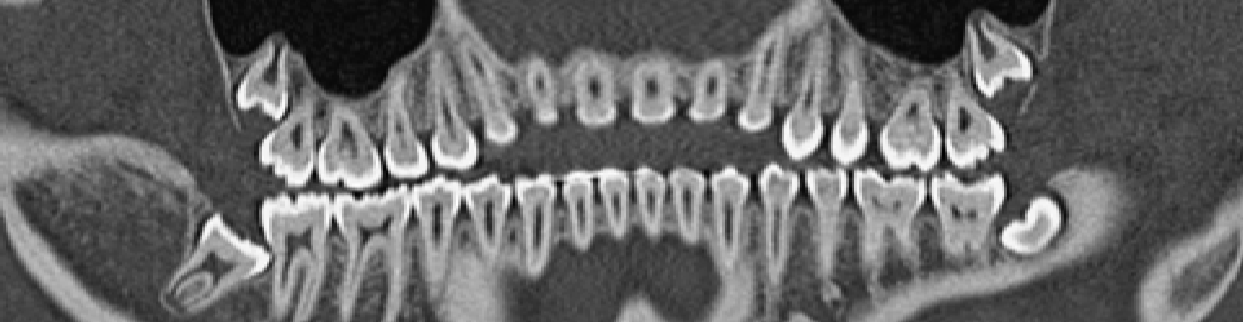
\includegraphics[width=0.8\textwidth]{Images/pano_paraview.png}
\end{figure}
%
\subsection{}

%
\section{Software Requirements}
%
\section{Conclusion}
%
%
\appendix

%%%%%%%%%%%%%%%%%%%%%%%%%%%%%%%%%%%%%%%%%
%
%  Insert the bibliography using BibTeX
%
%%%%%%%%%%%%%%%%%%%%%%%%%%%%%%%%%%%%%%%%%

\bibliographystyle{plain}
\bibliography{references}


\end{document}

